\subsection{home.web.cern.ch}

En este experimento se creo un paquete ICMP con dirección IP destino \textit{137.138.76.28}, correspondiente a la web \textit{http://home.web.cern.ch/} página oficial de la Organización Europea para la Investigación Nuclear (CERN). Los servidores de este sitio web se encuentran en la ciudad de Ginebra, Suiza. Se espera por lo tanto que a lo largo del camino que tome el paquete haya un salto transoceánico entre dos routers que obtendrá un alto puntaje según el z-score. Veamos primero una lista de las IPs junto a los lugares físicos asociados a esta para visualizar con mayor facilidad el recorrido que realizó el paquete a lo largo del experimento:

\begin{figure}[H]
  \centering	
	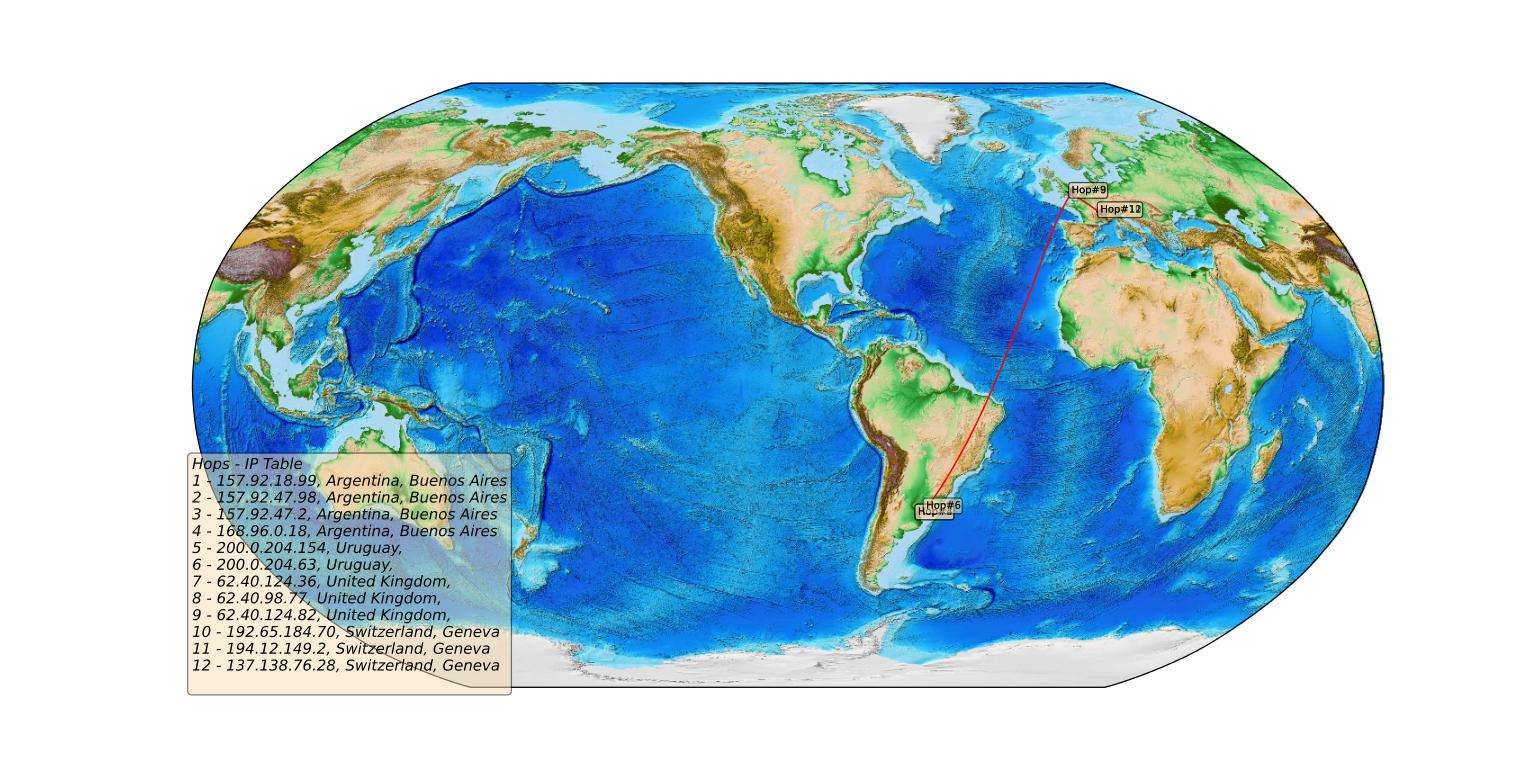
\includegraphics[scale=0.3]{../cern-experiment/figure_1.jpeg}
  \caption{Mapamundi con un croquis del viaje realizado por el paquete en rojo.}
	\label{fig:histo-src-sitiotrabajo}
\end{figure}

Como se puede ver el \textit{hop} entre el sexto y septimo router es el transoceánico del que se habló anteriormente. El salto se produce entre Uruguay (\textit{200.0.204.63}) y el Reino Unido (\textit{62.40.124.36}). En el siguiente gráfico, que muestra el RTT entre dos routers consecutivos medido en milisegundos, el salto que arriba al Reino Unido es el que devuelve el valor más alto. Esto tiene sentido ya que este es el de mayor distancia geográfica.

\begin{figure}[H]
  \centering	
	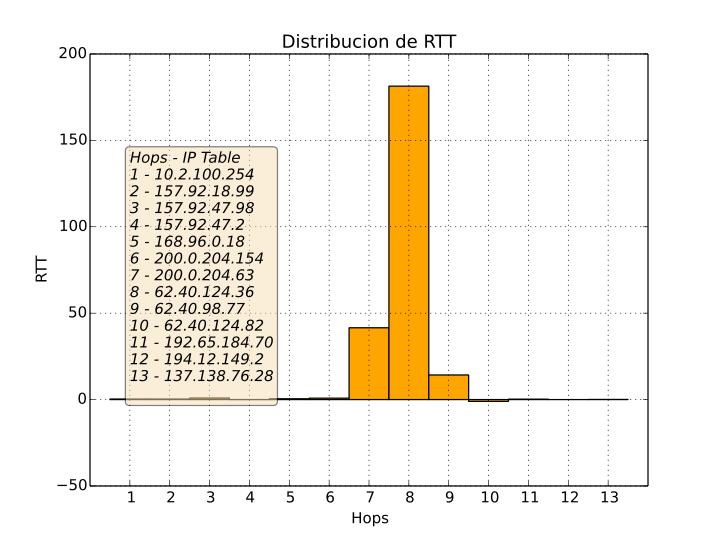
\includegraphics[scale=0.3]{../cern-experiment/bar_rtt.jpeg}
  \caption{RTT entre dos router consecutivos medido en milisegundos.}
	\label{fig:histo-src-sitiotrabajo}
\end{figure}

\begin{figure}[H]
  \centering	
	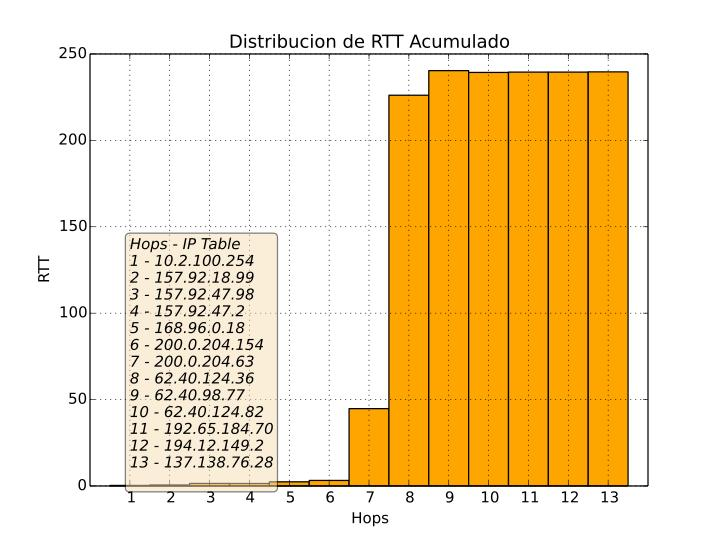
\includegraphics[scale=0.3]{../cern-experiment/bar_rtt_acum.jpeg}
  \caption{RTT acumulado del paquete a medida que avanza en su camino hacia el host del CERN.}
	\label{fig:histo-src-sitiotrabajo}
\end{figure}

Finalmente, se pueden ver los resultados obtenidos con el \textit{z-score} donde se observan valores similares (en proporción) a los obtenidos en el primer gráfico de esta sección. Más aun, el puntaje fue negativo para aquellos saltos que pueden ser etiquetados como de menor importancia, aquellos que tienen un desplazamiento geográfico menor y en consecuencia no aportan demasiado al tiempo total de viaje del paquete. Entre los saltos destacados, se puede ver una diferencia más pronunciada a la hora de encontrar al octavo como \textit{hop} distinguido.

\begin{figure}[H]
  \centering	
	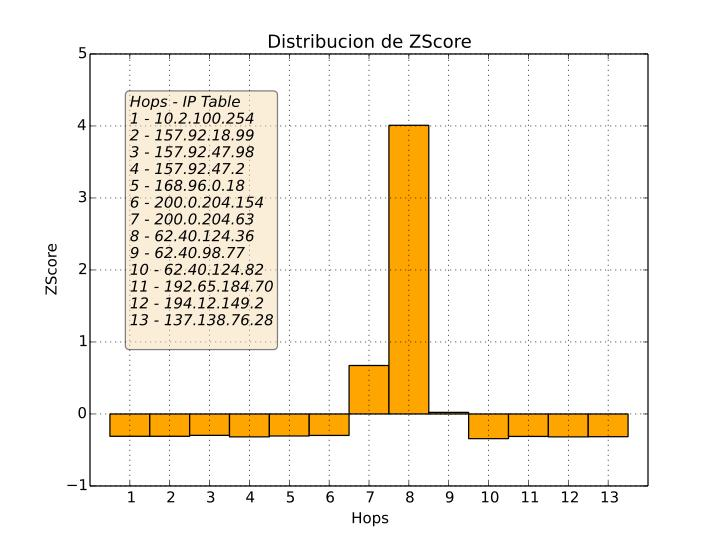
\includegraphics[scale=0.3]{../cern-experiment/bar_z_score.jpeg}
  \caption{Z-Score para cada uno de los saltos.}
	\label{fig:histo-src-sitiotrabajo}
\end{figure}
